% !TEX root = ../Dokumentation.tex
\section{Realisierung}

\subsection{RaspberryPi}

Folgende Installation \& Grundkonfigurationen müssen zu Beginn am RaspberryPi vorgenommen werden.

\subsubsection{Software}
Die 32GB grosse SD-Karte welche man für das Raspberry benötigt, wird zu Beginn formatiert um danach eine saubere Installation des Betriebssystems durchzuführen. Als OS wird die Version 2017-04-10 raspbian-jessie verwedent, dieses Betriebssystem wird von diversen Webseiten und Anleitungen empfohlen. Es hat eine graphische Oberfläche und bietet bereits vorinstallierte Programme.

\begin{figure}[H]%Position festigen
\centering
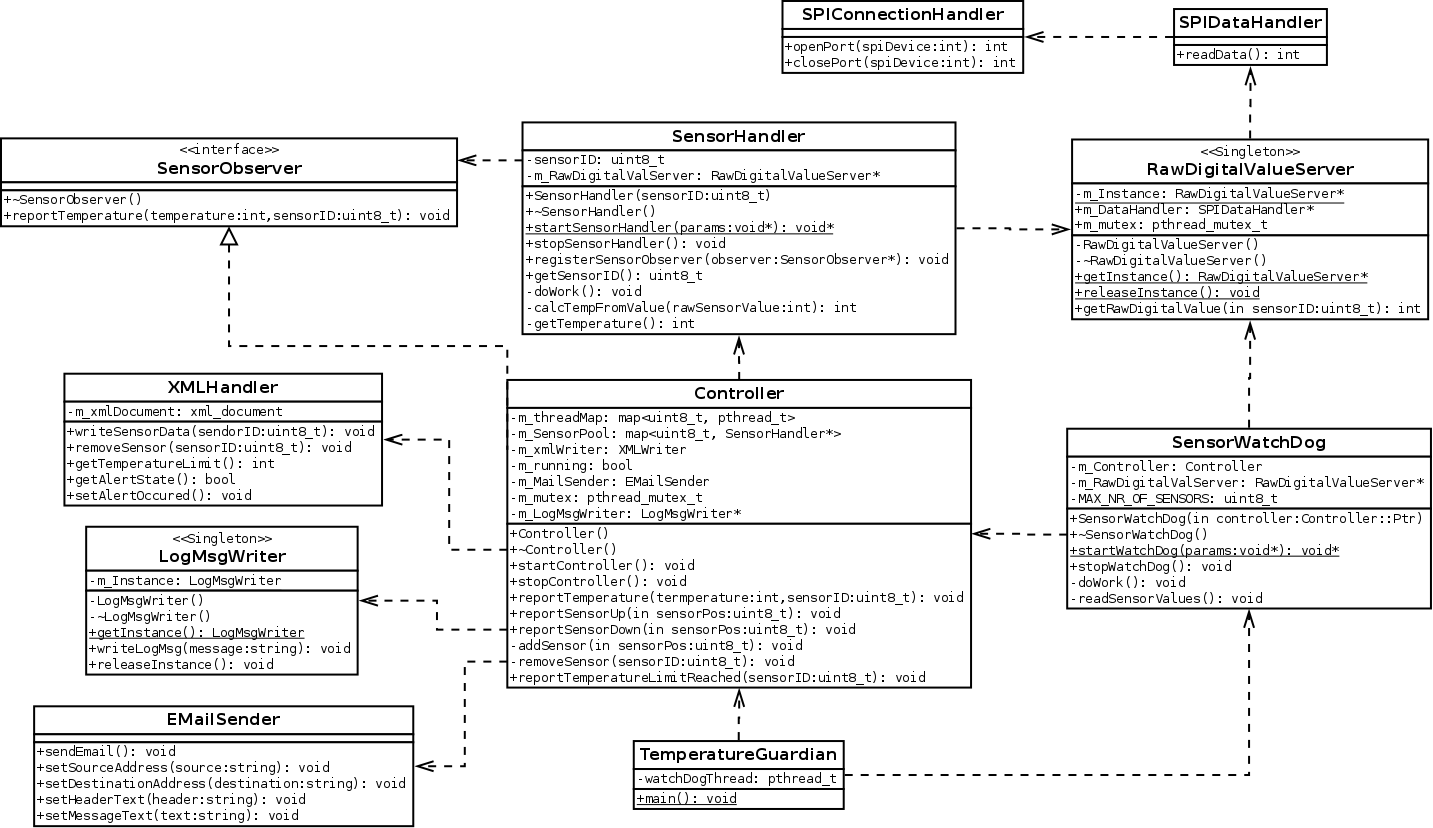
\includegraphics[width=1\textwidth]{Images/Klassendiagramm.png}
\caption{Klassendiagramm Software}
\label{fig:classdia}
\end{figure}

\subsubsection{Konfiguration}
Nach der Installation der Software kann das Raspberry mit Maus und Tastatur an einen Monitor angeschlossen werden. Sobald das Raspberry mit Strom versorgt wird, startet der Boot-Vorgang.
Nun müssen alle wichtigen Grundkonfigurationen wie folgt vorgenommen werden.

Tastatur: Deutsch(Schweiz)
Username: TemperatureSensorPi\\
Passwort: temperatur2017\\
Inteface SPI: enable\\
Netzwerk: <tbd>

\subsection{Softwaredesing}
\subsection{Verwendete Hardware}

\begin{figure}[H]%Position festigen
\centering
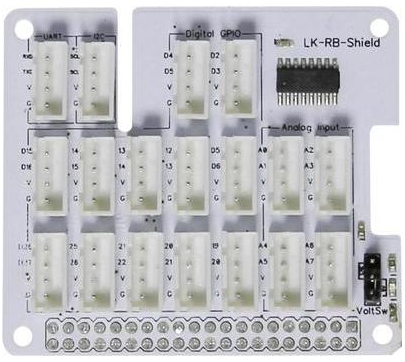
\includegraphics[width=0.25\textwidth]{Images/Basisplatine.jpg}
\caption{Basisplatine zum Raspberry Pi (Quelle www.Conrad.ch)}
\label{fig:plate}
\end{figure}

\begin{figure}[H]%Position festigen
\centering
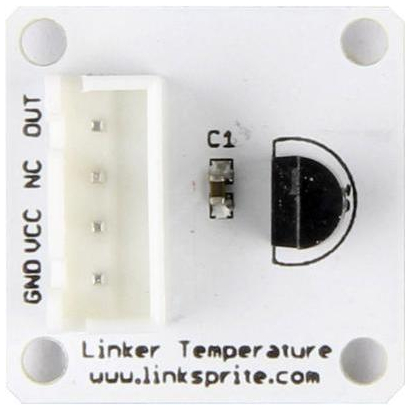
\includegraphics[width=0.25\textwidth]{Images/Sensorplatine.jpg}
\caption{Sensorplatine mit Temperaturfühler (Quelle www.Conrad.ch)}
\label{fig:sensor}
\end{figure}

\begin{figure}[H]%Position festigen
\centering
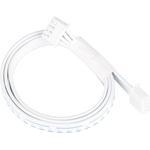
\includegraphics[width=0.25\textwidth]{Images/Verbindungskabel.jpg}
\caption{Verbindungskabel (Quelle www.Conrad.ch)}
\label{fig:cable}
\end{figure}

\subsection{Webdarstellung}

\section{Versuchsdurchführung}